\section{Durchführung}
\label{sec:Durchführung}

Es wird eine Kaliumbromid-Probe untersucht.

\subsection{Aufbau und Ablauf}
\autoref{fig:versuchsaufbau} zeigt den Versuchsaufbau. 

\begin{figure}[H]
    \centering
    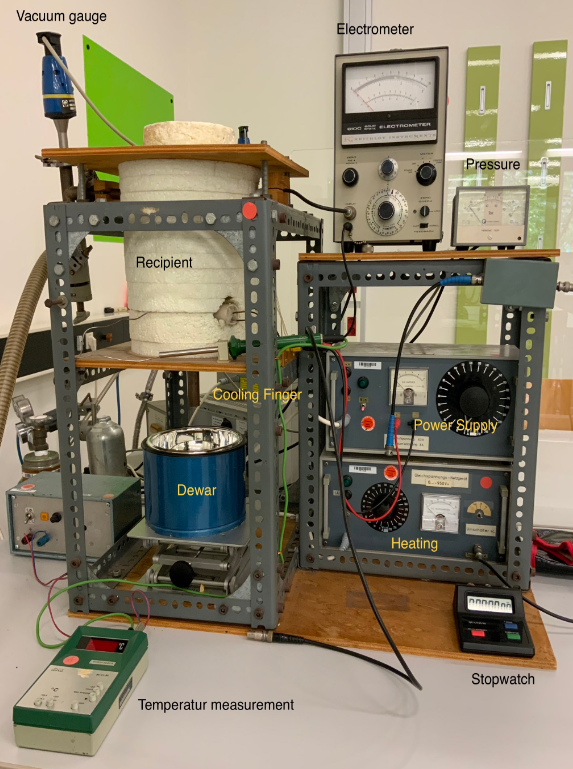
\includegraphics[width=\textwidth]{v48/Bilder/versuchsaufbau.png}
    \caption{Versuchsaufbau für Relaxationsprozesse in Ionenkristallen.}
    \label{fig:versuchsaufbau}
\end{figure}

Mit einer Drehschieberpumpe wird im Rezipienten, wo sich die Probe befindet, ein Vakuum von $\qty{10e-2}{\milli\bar}$ aufrechterhalten, damit das hygroskopische Salz vor insbesondere Luftfeuchtigkeit 
geschützt ist, die die Messung beeinflusst. Die Probe liegt auf einer Platte mit einem Kühlfinger auf, der aus dem Rezipienten rausragt und für die Kühlung in einen mit flüssigen Stickstoff gefüllten Dewar geführt werden kann.
Um die Probe zu erhitzen, ist eine Heizwicklung im Rezipienten verbaut. Für die Temperaturmessung ist des Weiteren ein Thermometer verbaut.
Um die Probe zu polarisieren, liegt eine weitere Metallplatte auf der Probe, die mit der Auflageplatte des Kühlfingers einen Plattenkondensator bildet. Für die Strommessung wird der Plattenkondensator
umverkabelt und an ein Elektrometer angeschlossen.

Zu Beginn einer Messung muss die Probe auf bis zu $\qty{50}{\celsius}$ erwärmt werden, damit gewährleistet ist, dass möglichst viele Dipole sich entlang des elektrischen Feldes ausrichten können.
Bei dieser Temperatur wird für $\qty{900}{\second}$ ein elektrisches Gleichfeld mit einer Spannung von ungefähr $\qty{950}{\volt}$ aufgebaut. Der Dewar wird mit flüssigem Stickstoff gefüllt und der Kühlfinger
in die Flüssigkeit eingetaucht, bis die Probe eine Temperatur von ungefähr $\qty{-50}{\celsius}$ hat. Das elektrische Feld wird abgeschaltet und der Plattenkondensator für weitere $5$ Minuten kurzgeschaltet,
um ihn zu entladen. Danach wird das Elektrometer und das Heizelement angeschlossen. Zwischen der Starttemperatur $T_0 = \qty{-50}{\celsius}$ und der Endtemperatur $T_\text{end} = \qty{30}{\celsius}$ wird minütlich die Temepratur und der Strom gemessen.

\subsection{Tatsächliche Durchführung}

Es wurden zwei Messreihen mit zwei verschiedenen Heizraten, d.h. mit zwei verschiedenen Heizspannungen, durchgeführt. Die erste Erhitzung beider Messreihen lief, bis die Probe ungefähr $\qty{55}{\celsius}$ hatte, wobei das Gleichfeld angeschaltet wurde, als die Probe ungefähr $\qty{40}{\celsius}$ heiß war.
Das Feld wurde während der Abkühlung ausgeschaltet und die Platten bei ungefähr $\qty{-45}{\celsius}$ kurzgeschlossen. Die Starttemperatur betrug in beiden Fällen $\qty{-60}{\celsius}$. Für die erste Messreihe wird eine Heizspannung von ungefähr $\qty{70}{\volt}$ eingestellt, für die zweite eine von ungefähr $\qty{80}{\volt}$. 
Mit einer Stoppuhr wurde minütlich die Temperatur und der Strom gemessen, wobei die beiden Messungen aufgrund der Zeit zum Ablesen
des sensiblen Picoampèremeters nicht zeitgleich stattfanden, sondern mit einem Abstand von ungefähr $10$ Sekunden. Die Endtemperatur betrug in beiden Fällen ungefähr $\qty{20}{\celsius}$.